\chapter{Soft Materials Modelling: Artificial Neural Networks} 
\label{ch6:ANN}

\section{Introduction} 

In the previous chapter, the development of two mathematical models for the prediction of viscoelastic behaviour in soft materials is described. The PL-SLS model and the PL-Wiechert model can describe the nonlinear, time dependent, and strain dependent stress response of seven soft materials. The main limitation of modelling tools based on mathematical models is their implementation in control systems for real robotic applications. Due to this, a different modelling approach is investigated in this chapter.

The field of machine learning provides reliable algorithms to tackle regression problems, such as artificial neural networks (ANNs). ANNs have been successful in extracting complex mechanical parameters of soft materials, and are now being used to model the stress-strain curve of many materials. Nonetheless, back in 2016 the literature on the latter subject was very scarce. It is until 2019, that a surge in research dealing with the implementation of different architectures of ANNs, in combination with Dynamic Mechanical Analysis (DMA), is being performed as an attempt to model the viscoelastic properties of soft materials. Nonetheless, there is still plenty of research to be done, such as implementing ANNs for the real-time prediction of the viscoelastic properties of soft materials. In this context, real-time prediction refers of deploying the trained ANN model into a control system, essentially replacing the mathematical model commonly used to estimate the stress-strain curve of elastic elements used in series-elastic actuators. This gap in the body of knowledge is addressed in this research.

%The field of machine learning provides reliable data-driven modelling tools, such as artificial neural networks (ANNs). ANNs have been successful in extracting complex mechanical parameters of soft materials, and are now being used to model the stress-strain curve of many materials. Back in 2016, the literature about the characterization of soft materials properties using ANNs was very scarce. Specifically, literature investigating the potential of ANNs of modeling the viscoelastic behaviour of soft materials was nonexistent. Very recently, there has been an increase in the popularity of the latter subject, an example of this is the work from REF. The authors make use of DMA to extract the viscoelastic properties of a soft material. Then, these data is used to train a ANN model which is aimed to describe the relationship between the strain, the stress, the strain rate, and the temperature of soft materials. 

In this work, a feedforward ANN model is developed. The Bayesian Regularization algorithm is used during the training process. The selection of inputs and outputs to be included to the network is optimized by observing the generalization capabilities of different combinations. The total number of neurons in the hidden layer is also optimized to minimize the risk of a common phenomenon known as over-fitting. The optimal number of neurons varies from one soft material to the other, but in any case exceeds 10 neurons.

Finally, the generalization error of the developed ANN is compared against the PL-SLS and the PL-Wiechert models. The results varies from one material to the other. In general, the developed ANN model can predict the nonlinear time-dependent stress response of the soft materials. The ANN model performed poorly for the single case of the NatR material. The reasons behind this might be related to the uneven dataset of this material. Lastly, the three developed modelling tools so far are suitable for the prediction of the complex behaviour of soft materials.

\section{Artificial Neural Networks}

Artificial Neural Networks (ANNs) are computational systems inspired in the structure and functionality of the biological nervous system. Neurons, a specific type of cell, are the basic components in the brain. They form connections with a vast number of other neurons, allowing us to remember, think, and apply previous knowledge to our present actions. The basic functionality of a neuron is to receive information in its inputs from many sources, to combine this information, to apply a nonlinear operation, and to output the end result. Moreover, neurons are capable of specializing for a specific task by amplifying or reducing the impact of their individual inputs. Neurons are also capable of reorganizing themselves in complex interconnected clusters in a three-dimensional space, called biological neural networks, where the information flows from one group of neurons to the other.

Similarly, Artificial Neural Networks are composed of many basic components working in parallel, known as artificial neurons. The clustering found in biological neural networks, can be replicated in ANNs by creating layers, containing many neurons, which can be interconnected between each other in different ways. The simplest structure of an ANN is composed of three layers: an input layer, a hidden layer, and an output layer. As the name suggest, the input and output layers interface the ANN with the outside world. The main learning process happens in the hidden layer. The way in which the interconnections between these three layers are formed are mainly dependent on the application. The strength of each interconnection depends on a weighting factor, enabling the artificial neuron to amplify or reduce the contribution of a specific input. The fine tuning of these weights, performed in a process called training, allows ANNs to specialize in a particular task, i.e. allow them to learn. The latter highlights the capability of ANNs to simulate two key functionalities of the human brain, which are: acquiring knowledge from the environment through a learning process, and storing this knowledge in the form of inter-neuron connection strengths, i.e. synaptic weights. The capability of learning from experience, i.e. experimental data, make ANNs particularly useful when dealing with complex scientific and engineering problems where an adequate analytical description is not available, or is too complex  \cite{zhang2003artificial,trebar2007predicting}.

Artificial Neural Networks can have as many layers as required, simulating the clustering phenomenon found in biological neural networks. These type of multi-layered ANNs can be categorized depending on how the information flows inside it. For example, an ANN in which the information flows in one direction, from the input layer up to the output layer, is called Feedforward Neural Network (FFNN). This type of ANN is one of the most commonly used for function approximation, pattern recognition and classification (\Cref{fig:FFANN}) \cite{zhang2003artificial}.

\begin{figure}[htb!]
	\centering
    \begin{subfigure}[b]{0.49\textwidth}
        \centering
        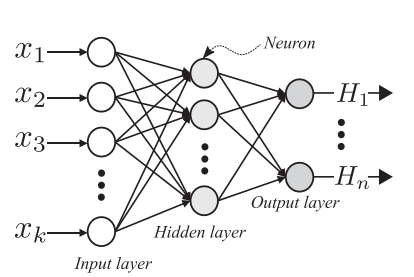
\includegraphics[width=\textwidth]{FeedForwardANN.PNG}
        \caption{}
        \label{fig:FFANN}
    \end{subfigure}
    \begin{subfigure}[b]{0.49\textwidth}
        \centering
        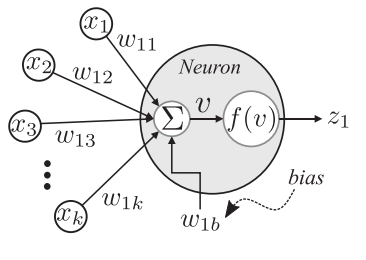
\includegraphics[width=\textwidth]{Neuron.PNG}
        \caption{}
        \label{fig:neuron}
    \end{subfigure}
    \caption[(a) Feedforward artificial neural network (b) Internal structure of an artificial neuron.]{(a) Feedforward artificial neural network (b) Internal structure of an artificial neuron \cite{rodriguez2019application}.}
    \label{fig:neruonANN}
\end{figure}

The variables illustrated in \Cref{fig:FFANN} are as follows. The inputs of the ANN are represented by the variable $\mathbf{x}$, in the form of:

\begin{equation}
    \mathbf{x} = [x_1, x_2, x_3, ... , x_k ]
    \label{c6_neuronin}
\end{equation}

\noindent where $k$ represents the total number of inputs. Similarly, the outputs of the ANN are represented by the variable $\mathbf{H}$ in the form of:

\begin{equation}
    \mathbf{H} = [H_1, H_2, H_3, ... , H_n ]
    \label{c6_networkout}
\end{equation}

\noindent where $n$ represents the total number of outputs. Furthermore, the output of the neuron illustrated in \Cref{fig:neuron}, combines the individual weighted values of the input vector $x$ with a bias value. Then, a nonlinear function is applied to the result of this sum. This is described as follows:

\begin{equation}
    z_1 = f \left( \sum_{i=1}^k(x_i w_{i,j}) + w_{1,bias} \right)
\label{c6_neuronout}
\end{equation}

\noindent where $w_{1,1}$ to $w_{1,k}$ represents the weights of one neuron which interacts with all the inputs. The subscript $i$ in $w_{i,j}$ indicates to which neuron this weight is interacting, whereas the subscript $j$ indicates the input that this weight is related to.

In order for the ANN to learn, it must be trained first. In FFNN the most common approach for training is based on the backpropagation algorithm. The training process of ANN commonly involves dividing the available data into a training and a test subset. The former subset is used for training of the ANN, whereas, the latter is used for testing the prediction capabilities of the ANN after being trained. During training, the ANN is presented with known values of the output, called targets, which are related to a specific combination of inputs. In each training session the ANN will adapt slightly until its output is close to the target value. The backpropagation algorithm is based on minimizing the sum of square errors (SSE) between the target and predicted values, by modifying the weights and biased of the ANN \cite{zhang2003artificial}. This algorithm is so powerful in minimizing the error that it could cause the ANN to memorize the training dataset instead of generalizing it. This means that the ANN will not be able to provide accurate predictions when new data is presented to it. This issue is called over-fitting.

According to the literature, FFNN are capable of representing any functional relationship between a set of inputs and outputs, as long as the ANN has enough number of neurons in its hidden layers. However, having too many neurons increases the risk of over-fitting. As previously mentioned, over-fitting will prevent the ANN to generalize well. Therefore, when designing an ANN, it is better to use the minimum amount of resources which are able to provide a good fit. There are two main methods for preventing over-fitting from happening, i.e. improving generalization, during the training process: early stopping and regularization. On the one hand, in the early stopping method, a third subset of data is involved, called the validation subset. In general terms, when the error during the validation process increases over certain number of consecutive training sessions, then over-fitting is detected and the training process is stopped. On the other hand, in a regularization method the performance function used during training, commonly the SSE of the ANN prediction, is modified. For example, in the Bayesian Regularization method, the performance function has an additional condition, which is to minimize the SSE of the weights and biases of the ANN. This limits the correction power of the backpropagation algorithm, which allows the weights and biased to be fine-tuned rather than have large variations. There are many variables involved in the process of designing and optimizing an ANN for a specific application. Therefore, the relevant works on implementation of ANNs for the modelling of soft materials are presented in the following section.

\section{Soft Materials Modelling }

Artificial Neural Networks have been implemented in a wide number of applications, such as: forecasting, control, power systems, robotics, signal processing, manufacturing, pattern recognition and optimization \cite{khan2019fabrication}. At the time of writing this document, the available literature about the implementation of ANNs for the modelling of the complex behaviour of soft materials, specifically elastomers, is scarce. Recently there has been an increase in the number of published papers focusing on modelling soft materials using ANNs which highlights the relevance of this field of research.

One of the earliest works in this field is documented in \cite{zhang2002dynamic} by Zhang et al.. In here, a FFNN is developed to model the dynamic mechanical properties of short fibre reinforced materials. The trained ANN can predict the storage modulus and damping of the material for temperature values not used during the training process. Many properties of the material are provided as input to the network. The developed ANN had 25 neurons in its single hidden layer with a tan-sigmoidal transfer function, whereas the output layer had a linear transfer function. The Bayesian Regularization algorithm was used for training. The prediction capabilities of the ANN were assessed using the percentage of correct predictions, in which a prediction with an $R^2$ value greater than 0.9 is considered correct. The ANN was tested 50 times with a randomized test set each time. Moreover, the authors found a proportional relationship between the complexity of the parameters to model, and the amount of data required for training to achieve a good accuracy.

The review paper of Zhang et al. about the implementation of ANNs in polymer composite applications states that the available literature on the subject was scarce at that time \cite{zhang2003artificial}. Moreover, the documented applications ranged from modelling of the fatigue life of the material, to prediction of tribological and dynamic mechanical properties of composite materials \cite{zhang2002prediction,zhang2002dynamic}. This review paper provided very insightful evidence of the potential of ANNs for applications such as: design of new composite materials, optimization of the manufacturing process, and modelling the relationship between different manufacturing parameters. From the reviewed works, the authors were able to find a well defined sequence of actions which describes the process of implementing ANNs for the prediction of the mechanical properties of composite materials:

\begin{enumerate}
    \item \textbf{Data collection:} the first step in designing an ANN is to collect enough data from experimentation. On top of this, processing of the collected data, mainly to filter out noise, might be required.
    \item \textbf{ANN design and training:} the second step is to design the ANNs depending on the application at hand. This involves deciding on the best parameters to use, in terms of: number of neurons, number of hidden layers, training algorithm and neuron's activation function. Also, this step involves the training of the proposed ANN.
    \item \textbf{Test of the trained network:} this step is about assessing the prediction and generalization capabilities of the trained ANN. The former is commonly assessed by looking at the difference between predicted and experimental values, as a general rule, the lower the error, the better the prediction. The generalization of the network is assessed by statistical methods such as p-fold cross-validation and the coefficient of determination.
    \item \textbf{Use of the trained network:} the last step is to use the trained network to simulate new data or for prediction.
\end{enumerate}

The latter process highlights the large number of configurations available when tackling a modelling problem. Due to this, some works in the literature opt for a ``trial and error'' approach when investigating the potential of ANNs for a specific application. Nonetheless, many works do perform optimizations in more than one of the ANN hyper-parameters. For example, motivated by the limitations of traditional viscoelastic models, the viscoelastic behaviour of polymer composites is investigated by Al-Haik et al. in \cite{al2006prediction}. In here an ANN is developed to predict the stress relaxation characteristics of a polymer composite. The amount of data used in here is rather large, having 900 datasets covering different conditions of the stress relaxation process. The training algorithm used is the scaled conjugate gradient. In addition to this, the optimal brain surgeon algorithm is used to optimize the topology of the network. The latter algorithm assesses the contribution of each neuron to the final results, by removing neurons one by one. This process is also known as pruning. The developed ANN had two hidden layers with 45 and 39 neurons, respectively; and was successful in modelling the stress relaxation characteristics of the material for ranges in which viscoelastic models were unsuccessful.

Initial works on this field of research were solely focused on one specific material. However, as the research matured, more materials were studied in a single work. This is the case for the work from Trebar et al. where a total of 12 different composite materials, natural rubber among them, were studied \cite{trebar2007predicting}. This work is more oriented towards assessing the generalization capabilities of ANNs for this specific selection of materials, having the previous knowledge of ANNs being successful for the modelling of viscoelastic materials. Therefore, more attention is given to the validation of the ANN prediction. This is done by using three different statistical parameters: (i) the root mean square error (RMSE), (ii) the normalized to the standard deviation, (iii) the mean absolute percentage difference (MAPE), and  (iv) the percentage of correctly classified samples. In this case, the Levenberg-Marquardt algorithm, an early stopping method, was used to prevent over-fitting. The dataset was divided into training (80\%) and testing (20\%) subsets. The training subset was further subdivided, allocating 80\% of the data for the actual training and 20\% for the validation process required for the early stopping algorithm. Different number of neurons in the hidden layer were tested, ranging from three neurons to three times the number of inputs. The latter ratio has also been mentioned in \cite{zhang2003artificial}, where three to four neurons per input node are found to be the optimal ratio. Although this is more a suggestion rather than a rule. Trebar et al. assessed the impact of using raw and preprocessed data for the training process. The preprocessed data consisted of the statistical parameters of the mechanical properties used as input, such as the standard deviation and mean values. The authors found that the developed ANN was in agreement with the experimental data of studied mechanical parameters of hardness and tensile properties.

Current implementations of ANNs in this field are focused more on using the ANN as an alternative to current mathematical models for the prediction of the stress relaxation and stress-strain curves of the materials. For example, in \cite{saeidirad2013predictions}, the prediction capabilities of an ANN are compared against one of the LVMs, the Generalized Maxwell model, also known as the SLS model. A rather simple ANN was developed in here, having only one input, the time, and one output, the stress. The back-propagation with declining rate algorithm was used for training. The performance of the ANN was assessed by the total sum of squared errors (TSSE) and by commonly used statistical parameters, such as the RMSE and $R^2$ coefficient. The optimal number of neurons was found by trial and error, keeping the learning rate, momentum and total number of epochs constant. In this case, the logarithmic sigmoid function was chosen due to the compatibility with the stress relaxation behaviour. The main difference between the latter function and the tan-sigmoid function is that the former have an output range of $[0,1]$, whereas the latter range is [-1,1]. In another work, the SLS model is again compared to an ANN \cite{gao2015viscoelastic}. In this case, many hyper-parameters, such as the number of neurons, number of hidden layers, and activation function in the hidden layers, are optimized by trial and error. Particular attention is put to the activation function of choice, which are tan-sigmoid (tansig) and logarithmic sigmoid (logsig). All combinations of using the latter function for a single and double layer network were assessed. The combination of using logsig and tansig in a double layered network was found to be the most optimal. The assessment of the performance of the ANN is based on the training time, overall training error and maximum error. The ideal network would have these parameters at its minimum values. This approach of minimizing the number of resources of the ANN was previously mentioned as a way to avoid over-fitting. Lastly, both mentioned works are good examples of the potential of ANN of replacing traditional mathematical models for the prediction of the stress relaxation of soft materials.

The literature on ANNs for the modelling of the stress-strain curve of soft materials is very scarce and fairly recent, in comparison to the literature available for metals \cite{ altinkok2005use,setti2014artificial, jenik2017sequential}. Nonetheless, one of the earliest attempts of modelling the stress-train curve of non-metal materials is documented in \cite{yousef2011prediction}. In this work, polymer composite materials are studied. The ANN developed in here follows the same trend of using FFNN. However, the number of neurons and hidden layers are larger than in previous applications. In this work, up to three hidden layers and up to 45 neurons, are investigated. The aim of this work was to analyse the effect of polymer blending ratio in the stress-strain curve of these materials. Current mathematical models were only effective, for the previously mentioned task, inside the elastic range of the material. The developed ANN was capable of overcoming this limitation. Moreover, a logsig activation function was used, together with a backpropagation training algorithm. No information is given on the reasoning behind the selection of neurons and hidden layer, therefore a trial and error approach must have been adopted. 

More recent works specifically investigates the performance of ANNs for the modelling of soft materials such as elastomers and thermoplastic elastomers (TPEs). An example of this is documented in \cite{kopal2017modeling}. The aim of this work is to model the temperature dependency on the dynamic mechanical properties of TPEs. Therefore, the materials are characterized using a Dynamic Mechanical Analysis (DMA), which describes the stress response of the material on a range of frequencies or strain rates. Nonetheless, the study is focused on a single frequency of 1 Hz. This particular work is closely related to the research presented in this thesis. Therefore, the methodology implemented by the authors is of interest. The work focuses on thermoplastic polyurethanes (TPUs). Again, the FFNN architecture is chosen for the developed ANN. The temperature history is presented as input to the network, whereas the storage modulus, damping factor, and loss modulus are the desired parameters to predict. Three individual ANNs were developed, one for each parameter. The latter parameters describes the viscoelastic properties of materials. In terms of the activation functions, the commonly used configuration of having a tangent-sigmoid function in the hidden layer and a linear function (purelin) in the output layer is chosen. The Levenberg-Marquardt back-propagation minimization algorithm was implemented. No particular measurements, besides the already provided by the training algorithm, were implemented to ensure good generalization capabilities of the network. Among the three developed ANN, no more than 15 neurons were used.

Kopa et al. continued the latter research in a recently published paper \cite{kopal2018prediction}, this time focusing on predicting the uni-axial tensile response of vulcanized rubber. Again, a FFNN is developed. The inputs were the engineering strain and the content of carbon black in the rubber blend. The output was the engineering uni-axial stress. The optimal number of neurons was found by trial and error, being six the optimal number of neurons. Similarly to previous applications, the tansig-purelin combination of transfer function was chosen. The Levenberg-Marquardt algorithm was also used. The main contribution of this work is the validation approach implemented, which is based on knowing the relationship between the material stress-strain ultimate values, and the carbon black content of the material. A quadratic regression can describe the latter with adequate accuracy. This is a simpler approach in comparison to fit the whole stress-strain curve of a material with a LVM. In summary, the ANN was presented with unknown values of carbon content, obtained from the regression model. The validation was successful since the ANN was capable, not only of agreeing with the ultimate strain-stress values corresponding to that carbon black content, but also of describing the whole stress-strain curve.

Lastly, the most recent work on this research field was performed by Rodriguez et al. in \cite{rodriguez2019application}. Many thermoplastic elastomers are studied in this work. Their stress/strain curves are extracted from an available dataset, hence no mechanical characterization is performed. The developed ANN is aimed to model the stress-strain curve of many thermoplastic elastomers under different values of temperature. In comparison to previous works, several optimizations are performed in this one. For example, the training process of the ANN consist of two steps. Initially, the Simulated Annealing (SA) algorithm is used to explore initial solutions for the weights of the network prior to applying the greedy gradient-based Levenberg-Marquardt (GGLM) algorithm. The main objective of the SA algorithm is to prevent the weights, tuned by the GGLM algorithm, to fall into a local minimum. The latter is a well-known side effect of Levenberg-Marquardt-based algorithms. Furthermore, the ANN developed in here is a FFNN with 10 neurons in its single hidden layer. The process of finding the optimal number of neurons involved the training and test of many ANNs with different number of neurons ranging from 1 to 20 neurons. The decision of using 10 neurons is based on the small improvement of the achieved prediction error when further increasing the number of neurons. No explicit mention of the activation function used in either of the ANN layers is given. The authors opted to use the Neural Lab software to developed the ANN, instead of the commonly used Neural Network Toolbox from Matlab\textregistered{}. The temperature and strain values were used as inputs, and the stress response as output. This work implements similar methods as the one found in the literature for data division, measurement of performance, and validation of the ANN prediction capabilities. Nonetheless, the validation process implemented is extensive because five different hyper-elastic models, and a Probabilistic Neural Network are used for comparison. The validation process was mainly focused on the prediction error rather than the generalization capabilities of the developed ANN. The latter was assessed using the Normalized Absolute Difference (NMAD) and the $R^2$ coefficient. An extra validation step was performed which consisted of retraining the ANN using the data from another material from the same type. In this case, the prediction error was slightly higher but still adequate, considering that no further optimizations were performed in this test.

Summarizing, the implementation of ANNs for the modelling and prediction of soft materials, such as composite materials, is still in its early stages. The available literature is very limited for the specific application of modelling the stress-strain curve of soft materials. Available works are focused on the effect of the temperature. Moreover, works focusing on the effect of the strain rate, hence the velocity-dependency, of the stress response of the soft materials are currently not available in the literature. The latter is addressed in this thesis. Nonetheless, the potential of ANNs for this application has been proven in the documented works. Despite the many differences in the selection of hyper-parameters for the developed ANNs, the architecture of choice has been the same, feedforward neural networks. Moreover, a very comprehensive review can be found in \cite{paliwal2009neural} which includes information about the commonly used validation methods, measurement of performance, sample size, and the type of statistical models, implemented in engineering applications. More detailed information on the specific statistical methods for the validation of the developed ANN, such as the p-fold cross-validation method can be found in \cite{wang2007review,koskela2003neural}

%It is important to mention that by the time of doing this research, the latter article was not available in the literature. As previously mentioned, the implementation of ANN in the area of polymeric materials and rubbers is limited.

%The authors states that at least two hidden layers are required to approximate any function to an arbitrary order of accuracy, and that one hidden layer is enough to approximate a bounded continuous function to arbitrary accuracy. The developed ANN was used to 

%In conclusion, ANNs or neural constitutive models have the potential to be a viable alternative to theoretical constitutive models for nonlinear viscoelasticity. A properly trained ANN model can easily be stored in a hand-held computer and be used by an engi- neer to predict reliably and efficiently the time-dependent mechanical behavior of a visco- elastic or a viscoplastic material. The ANN approach can determine the material parameters in any general constitutive model, however complex, learn from it and supplant it. It can also directly learn from experimental data, reproduce it to prescribed accuracy (bounded by the data), and predict beyond the range of training.


\section{Model Development}

As previously discussed in \Cref{ch2:Literature}, modelling the nonlinear, time dependent, and strain dependent stress response of soft materials is critical for the implementation of reliable control systems in soft robotic applications. This has been attempted in many ways, and is also attempted in this thesis with the development of the PL-SLS and the PL-Wiechert models described in \Cref{sec:ChapterModellingLVM}. The obtained results highlight the capabilities of these models of predicting the mechanical behaviour of soft materials. Nonetheless, the main limitation of modelling tools based on mathematical models is the high complexity required to achieve adequate accuracy. The latter is amplified when these models are deployed in hardware with limited computing power. This situation is not present in machine learning models where the high computational complexity happens during training only. The computational cost of a deployed model is minimum.

In line with the work available in the literature, a feed-forward back-propagation neural network is developed in here. Nonetheless, the optimization of many of its hyper-parameters is performed to increase its generalization capabilities. These hyper-parameters include: the number of neurons in the hidden layer and the selection of inputs. The remainder hyper-parameters used in here are based on successful implementations from the literature. \Cref{tbl:ANN_parameters} provides a summary of the hyper-parameters to be optimized and the hyper-parameters chosen based on the literature.

\begin{table}[!htb]
    \centering
    \caption{Summary of proposed and optimized hyper-parameters.}
    \begin{tabular}{l l}
    \toprule
    \multicolumn{2}{l}{Proposed Hyper-parameters} \\
    \hline
    Topology                         & Feedforward Neural Network \\
    No. of Hidden Layers             & 1 \\
    Hidden Layer Activation Function & Hyperbolic Tangent Sgimoid (tansig)\\
    Output Layer Activation Function & Linear (purelin)\\
    Training Algorithm               & Bayesian Regularization (BR)\\
    Cost Function					 & Mean Squared Error (MSE)\\
    Output                           & Stress ($\sigma$)\\
    Dataset Size                     & All available data\\
    Dataset Division Function        & Random Division  \\
    Validation Error Measurement     & Normalized Root Mean Squared Error (NRMSE)\\
    Validation Method                & Multiple Training Sessions (5)\\
    \midrule
    \multicolumn{2}{l}{Optimized Hyper-parameters}\\
    \hline
    Number of Neurons            & 1 - 20 \\
    Inputs                       & 1 - 3 \\
    \bottomrule
    \end{tabular}
    \label{tbl:ANN_parameters}
\end{table}

In this work, the training function \texttt{trainbr} is used to train the ANNs, which is based on the Bayesian Regularization (BR) algorithm. This is one of the two most commonly implemented methods to avoid overfitting in ANNs. The BR algorithm is more computational demanding than the Levenberg-Marquardt algorithm, which is commonly implemented as an early stopping training algorithm. Nevertheless, the BR algorithm performs better for function approximation applications, and when the dataset is small \cite{matlab2019improve}. These characteristics are inline with the dataset used in this research. The characteristics of the available dataset for each material is presented in \Cref{tbl:ANN_nueronOptData}.

\begin{table}[htbp!]
	\centering
	\caption{Total number of training samples per soft material for the number of neurons optimization. In here, the total number of training samples represents the 100\% of the whole dataset.}
	\begin{tabular}{lccccccc} \toprule
		Test Type		& EPR	& FR 	& NatPolR 	& NR 	& PR 	& SR 	& NatR \\
		\hline
		50 mm/min		& 45294	& 11675 & 4675 		& 11592 & 8788 	& 24810 &  3768\\
		250 mm/min		& -		& 11675 & 2129 		& 10143 & 4735 	& 11578 &  124344\\
		500 mm/min		& 14154 & 8754 	& 425 		& 8694 	& 676 	& - 	&  41450\\
		\hline
		Total			& 59448 & 32104	& 7229 		& 30429	& 14199	& 36388	&  169562\\
		\bottomrule
	\end{tabular}
	\label{tbl:ANN_nueronOptData}
\end{table}

The analyses presented in the following sections summarizes the large exploration process, initially based on a trial and error approach, performed as part of assessing the capabilities of ANNs for the prediction of the viscoelastic properties of the soft materials included in this research. These tests provided with enough evidence on the capabilities of ANNs for the mentioned application. Lastly, the optimization processes performed to some of the ANN hyper-parameters are described in detail in the following sections.

\subsection{Analysis of the Model Inputs Selection}

The first hyper-parameter to optimize is the selection of inputs. For this application, in which the modelling of the velocity-dependent stress response of the material is desired, the decision to include both the strain and the strain rate as inputs of the ANN models, is made. However, in the scenario where the developed ANN is deployed as part of a control system in a real application, having a derivative term and the peaks associated with rapid changes in the input can cause the ANN model to behave unexpectedly. An alternative to circumvent this limitation without preventing the ANN model to learn the time-dependent properties of the stress response, is to use the current and past values of the strain as inputs, i.e. the strain history, allowing the network to learn the time dependency of the stress response without having to differentiate any input. The latter configuration describes a very basic form of a Recurrent Neural Network. 

In this work, both described scenarios are analysed. On the one hand, the proposed ANN architectures which have derivative terms in its inputs is considered rate-dependent. On the other hand, the ANN architecture which has current and past values of their inputs, instead of a derivative term, is considered rate-independent. The proposed combination of inputs used to create the ANN models studied in this section, are described in \Cref{tbl:ANNArchitectures}.

\begin{table}[htbp!]
    \centering
    \caption{Proposed ANN architectures. The architectures FFRI1, FFRI2 and FFRI3 are rate-independent, whereas the architecture FFRD4 is rate-dependent.}
    \begin{tabular}{lcccc}
    \toprule
                            & FFRI1               & FFRI2                   & FFRI3                   & FFRD4\\
    \hline
    \multirow{3}{*}{Inputs} & $\varepsilon_t$   & $\varepsilon_t$       & $\varepsilon_t$       & $\varepsilon_t$       \\
                            &                   & $\varepsilon_{t-1}$   & $\varepsilon_{t-1}$   & $\Dot{\varepsilon_t}$ \\
                            &                   &                       & $\varepsilon_{t-2}$   &                       \\
    \hline
    Output                  & $\sigma_t$        & $\sigma_t$            & $\sigma_t$            & $\sigma_t$            \\
    \bottomrule
    \end{tabular}
    \label{tbl:ANNArchitectures}
\end{table}

As previously mentioned, the inputs and outputs listed in \Cref{tbl:ANNArchitectures} must be presented to the ANN in the form described in \Cref{c6_neuronin,c6_neuronout}, yielding:

\begin{equation}
    \mathbf{X} = 
        \begin{bmatrix}
            \varepsilon_{t_1}  & \varepsilon_{t_2}       & \varepsilon_{t_3}      & ... & \varepsilon_{t_n} \\ 
            \varepsilon_{{t-1}_1}& \varepsilon_{{t-1}_2}  & \varepsilon_{{t-1}_3}  & ... & \varepsilon_{{t-1}_n} \\
        \end{bmatrix}
\end{equation}
\begin{equation}
    \mathbf{H} = 
        \begin{bmatrix}
            \sigma^{pred}_{t_1}  & \sigma^{pred}_{t_2}       & \sigma^{pred}_{t_3}      & ... & \sigma^{pred}_{t_n} \\ 
        \end{bmatrix}
\end{equation}
\begin{equation}
    \mathbf{T} = 
        \begin{bmatrix}
            \sigma^{exp}_{t_1}  & \sigma^{exp}_{t_2}       & \sigma^{exp}_{t_3}      & ... & \sigma^{exp}_{t_n} \\ 
        \end{bmatrix}
\end{equation}

\noindent where \textbf{X}, \textbf{H}, and \textbf{T} are the inputs, outputs, and targets matrices. The variables $\sigma^{exp}$ and $\sigma^{pred}$ represent the experimental and predicted values of the stress response of the material for a given strain, respectively. The subscript $n$ refers to the total number of samples in each matrix. The assessment of the best combination of input parameters is based on a 10-fold cross-validation approach which includes the execution of several training sessions. During each training session, up to 10 sessions, the training dataset is randomized prior to be presented to the ANN. Due to the 90-10 proportion used to create the training and test subset, the latter means that the ANN will learn from a different 90\% of the data and at the same time, it will be tested with a different 10\% of the data, at random. Also, the initial weights of the ANN are randomized in each training session. By default, the measurement of performance used during training is the mean square error (MSE). However, the normalized root mean square error (NRMSE), between the ANN prediction and the experimental data, is extracted from each training session and used for validation \Cref{eq2} \cite{bergstrom2015mechanics}. Finally, the generalization error is defined as the mean NRMSE value from all the training sessions. The architecture with the lowest generalization error is considered as the best candidate.

Due to the findings from \Cref{sec:ChapterModellingLVM}, where the performance of the developed PL-SLS and PL-Wiechert models can be correlated to the properties of the soft materials, i.e. highly elastic, viscoelastic or highly viscous, the decision to optimize the selection of inputs presented to the ANN on the remainder of the studied soft materials is made. In other words, it is not safe to assume a ``one fits all'' approach due to the differences between the materials properties. 

\begin{table}[htbp!]
    \centering
    \caption{Proposed parameters for the selection of best inputs}
    \begin{tabular}{l m{1cm} l}
    \toprule
    \multicolumn{3}{l}{Fixed Hyper-parameters} \\
    \hline
    Number of Neurons           & & 20 \\
    Dataset Size     			& & 10\% of available data\\
    Data Division               & & 90\% for training, 10\% for testing\\
    Error Measure               & & NRMSE and Generalization Error\\
    Validation Method           & & 10-fold Cross Validation\\
    \bottomrule
    \end{tabular}
    \label{tbl:ANN_InputSelParameters}
\end{table}

In \Cref{tbl:ANN_InputSelParameters}, the hyper-parameters chosen for this optimization are described. This is intended to isolate the impact of the different inputs presented to the ANN. Similarly, the impact of the amount of data used during training is isolated by using only 10\% of all the complete dataset previously described in \Cref{tbl:ANN_nueronOptData}. Subsequently, the data is divided into training and testing subsets, containing 90\% and 10\% of the data, respectively. The size of the testing set is based on the number of training session to perform, which is 10. The Matlab function \texttt{cvpartition} is used to obtain 10 nonstratified subsets of data which guarantees a unique subset of data is used for each training session. The testing subset is used to validate the generalization capabilities of the ANN when unknown data is presented to it. Similarly, a relatively large number of neurons is used in this optimization to avoid limiting the performance of the ANN models. Finally, the results are illustrated in \Cref{fig:ANNGen4,fig:ANNGenNatR}. The obtained charts indicates that the FFRD4 architecture is the one with the best generalization capabilities, i.e. smallest generalization error. In some cases, such as the EPR and NR materials, the achieved error of the FFRI1 and FFRD4 architectures are very similar. The difference between the achieved errors are minor. Hence, the FFRD4 architecture is selected as the best candidate.

Another important observation is the relationship between the achieved error and the complexity of the rate-independent architectures. In other words, presenting the ANN models with more inputs, in the form of past values of the strain, does not always yield in a performance increase. This is the case for the FR, NR, and SR materials. These results could be related to a weak velocity-dependency of the previously mentioned materials. Presenting the ANN models with additional inputs, aimed to account for velocity dependencies in the materials stress response, can harm the learning process rather than aid it.

\begin{figure}[htbp!]
	\centering
    \begin{subfigure}[b]{0.49\textwidth}
        \centering
        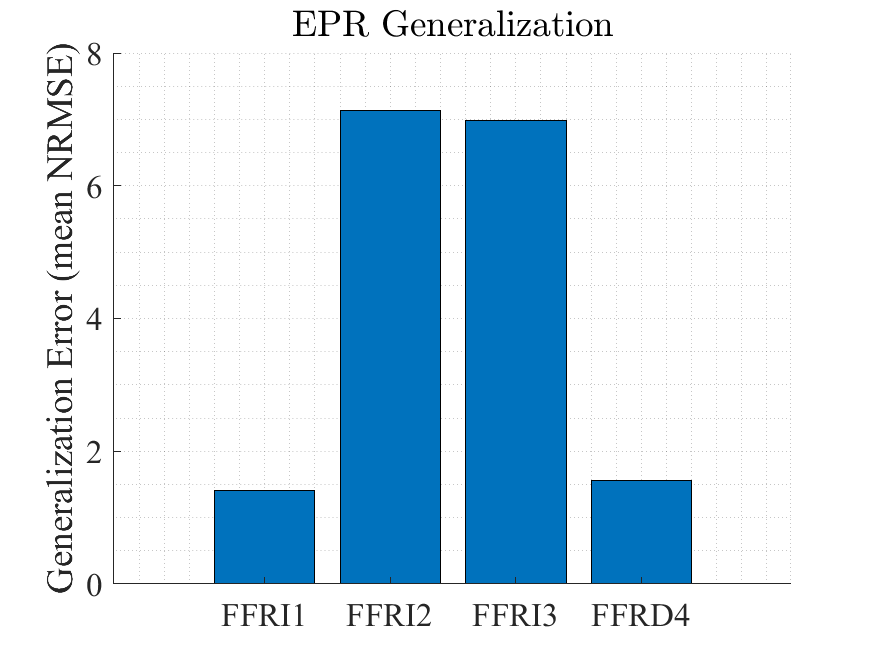
\includegraphics[width=\textwidth]{EPRANNGenECV.png}
        \caption{}
        \label{fig:ANNGenEPR}
    \end{subfigure}
    \begin{subfigure}[b]{0.49\textwidth}
        \centering
        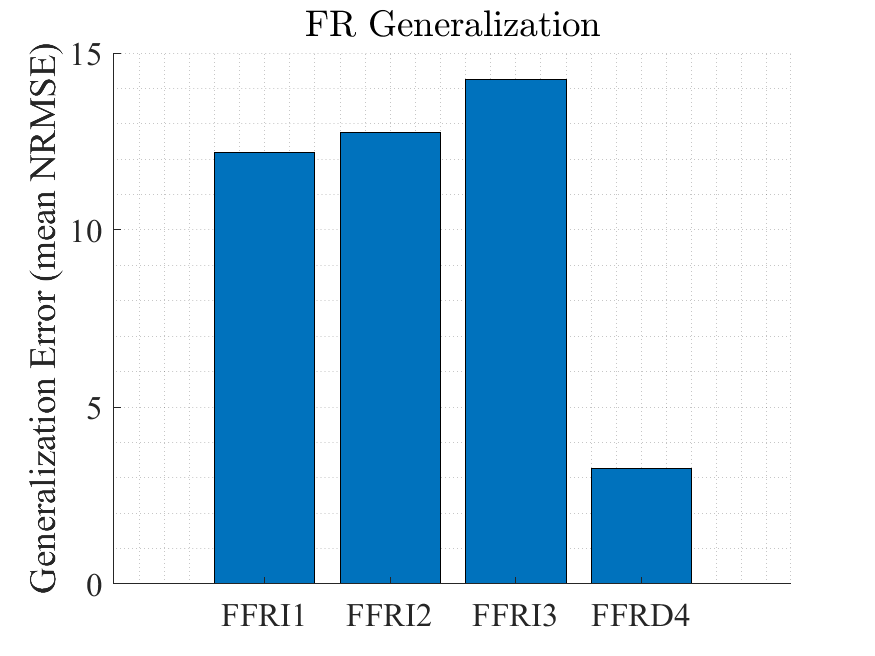
\includegraphics[width=\textwidth]{FRANNGenECV.png}
        \caption{}
        \label{fig:ANNGenFR}
    \end{subfigure}
    \begin{subfigure}[b]{0.49\textwidth}
        \centering
        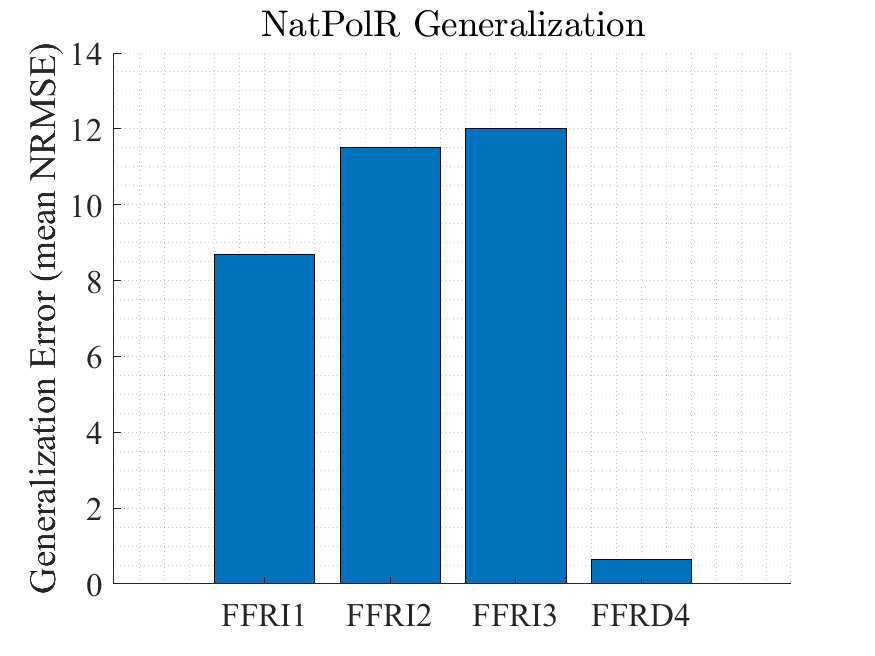
\includegraphics[width=\textwidth]{NatPolRANNGenECV.png}
        \caption{}
        \label{fig:ANNGenNR}
    \end{subfigure}
    \begin{subfigure}[b]{0.49\textwidth}
        \centering
        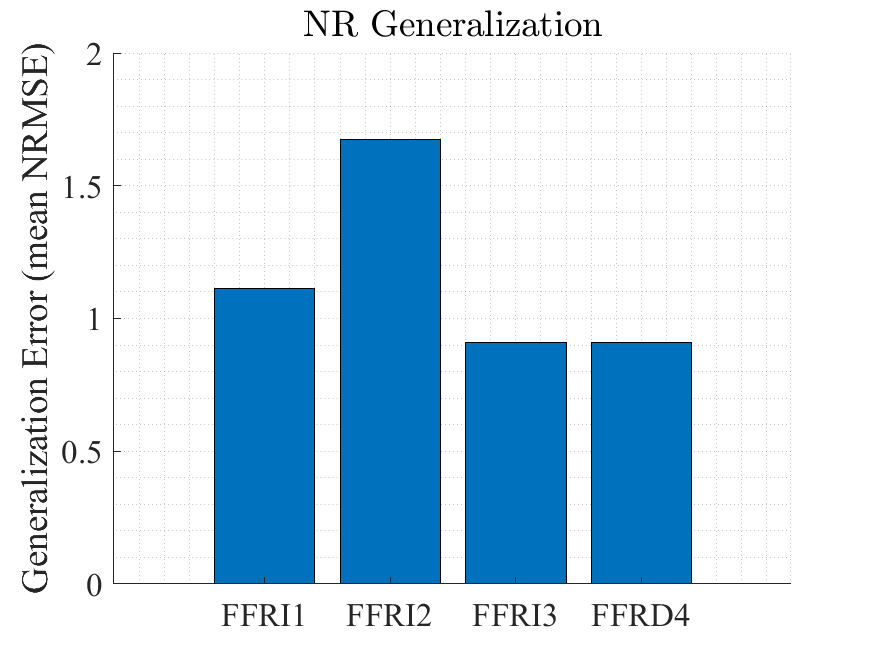
\includegraphics[width=\textwidth]{NRANNGenECV.png}
        \caption{}
        \label{fig:ANNGenNatPolR}
    \end{subfigure}
	\begin{subfigure}[b]{0.49\textwidth}
		\centering
		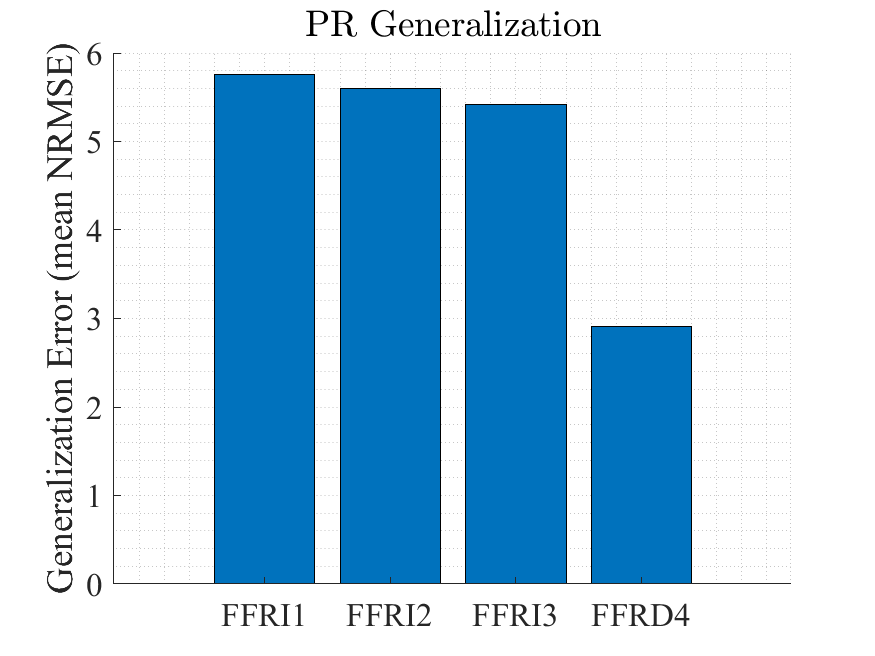
\includegraphics[width=\textwidth]{PRANNGenECV.png}
		\caption{}
		\label{fig:ANNGenPR}
	\end{subfigure}
	\begin{subfigure}[b]{0.49\textwidth}
		\centering
		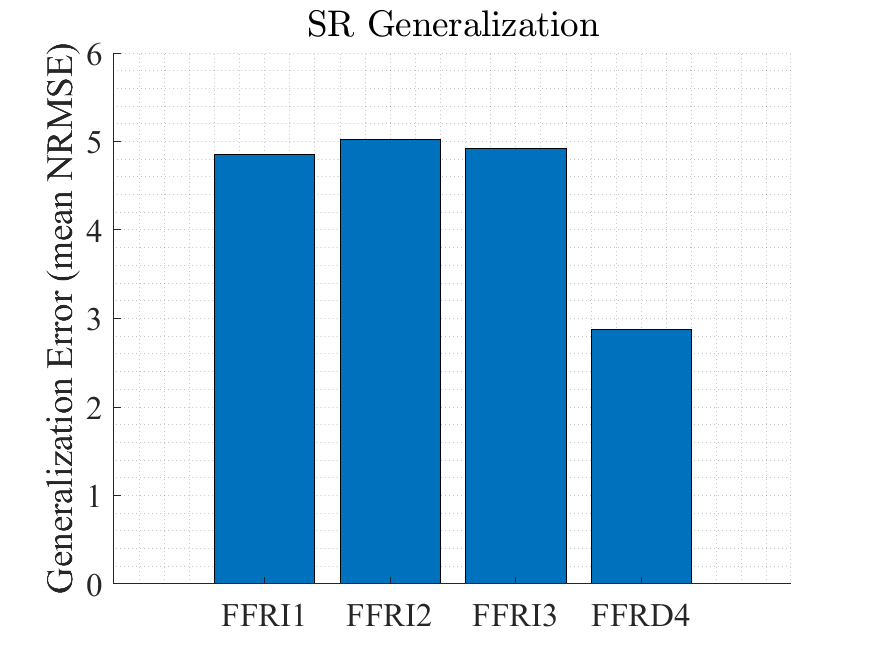
\includegraphics[width=\textwidth]{SRANNGenECV.png}
		\caption{}
		\label{fig:ANNGenSR}
	\end{subfigure}
    \caption{Generalization error, based on a 10-fold cross-validation, for the (a) EPR, (b) FR, (c) NatPolR, (d) NR, (e) PR, and (f) SR materials. The best input combination is the one with the smallest generalization error, which in most cases is the FFRD4 configuration.}
    \label{fig:ANNGen4}
\end{figure}

\begin{figure}[htbp!]
	\centering
	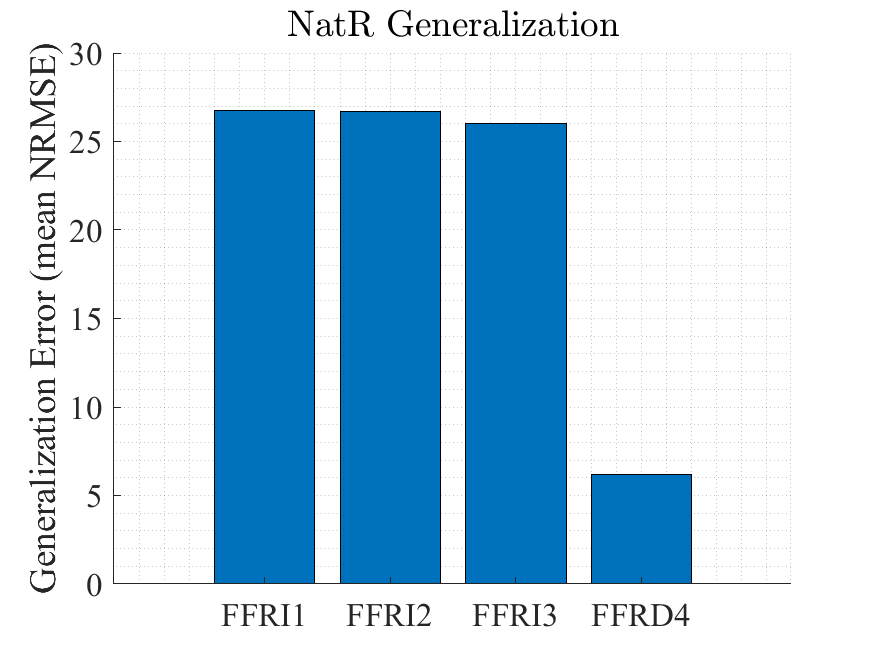
\includegraphics[width=0.49\textwidth]{NatRANNGenECV.png}
	\caption{Generalization error, based on a 10-fold cross-validation, for the NatR material. The best input combination is the one with the smallest generalization error, i.e. the FFRD4 configuration.}
	\label{fig:ANNGenNatR}
\end{figure}

As part of this analysis, the concept of having past values of the material stress response as input to the ANN model was also investigated. The achieved generalization error of this architecture is at least one order of magnitude lower than the other four architectures. Nonetheless, this concept is later dropped due to its incompatibility with a real robotic application. In other words, having the stress response of the material as input to the ANN model would translate into adding a load cell to the application. This cancels out one of the main benefits behind series-elastic actuators, which is transforming the force control problem into a position control problem. In other words, using a modelling tool to predict the stress response of the material based on the measured deformation of the material. Finally, the optimization performed in here showed that a rate-dependent architecture, such as the FFRD4, is more suitable for accounting the velocity-dependency of the stress-strain curve of soft materials.

\subsection{Analysis on the Optimal Number of Neurons}

In the literature, having two to three neurons for each input of the ANN is recommended. This recommendation seems to be in accordance to the number of neurons used in the documented implementations \cite{rodriguez2019application,kopal2018prediction,jenik2017sequential}. Nonetheless this is not true for all implementations \cite{yousef2011prediction,kopal2017modeling}. Moreover, the number of neurons must be kept at its minimum to avoid the ANN to over-fit the training dataset. Therefore, it is desirable to search for the optimal number of neurons which allows the developed ANN models to achieve a desired accuracy. In here, the latter search is performed, initially, for a range of 1 to 20 neurons. The coefficient of determination, $R^2$ value, is used to assess the performance of the ANNs. In addition to this a 10-fold cross validation is performed. The latter is done by firstly dividing the whole training dataset into 10 subsets. Then, multiple training sessions are performed. In each training session, 1 out of the 10 available subsets becomes the test set and the remainder 9 subsets become the training set. In this way, each training session use a different section of the whole dataset during the training. On top of this, the range from 1 to 20 neurons is investigated. This means, a total of 200 ANN models are training per soft material. The main objective of this optimization process is to limit the resources of the developed ANN models, i.e. to avoid over-fitting. The training session with the minimum number of neurons that has a value of $R^2>99.9\%$ is considered as the best candidate. A similar process to this, but using the percentage of correct prediction, is documented in \cite{zhang2002dynamic}.

In this optimization, the complete dataset available for each material is subdivided to allocate 90\% of the data for training and 10\% for testing. As previously mentioned, no validation subset is required when using the Bayesian Regularization algorithm. Therefore, the training set is no further subdivided. The list of hyper-parameters used in this case is compiled in \Cref{tbl:ANN_nueronOpt}, and the total number of training samples for each soft material is compile din \Cref{tbl:ANN_nueronOptData}.

\begin{table}[htbp!]
    \centering
    \caption{Proposed hyper-parameters for the number of neurons optimization}
    \begin{tabular}{l m{1cm} l}
    \toprule
    \multicolumn{3}{l}{Fixed Hyper-parameters} \\
    \hline
    Architecture               & & FFRD4 (see \Cref{tbl:ANNArchitectures})\\
    Number of Neurons           & & 1 to 20 \\    
    Error Measure               & & $R^2$ value\\
    Validation Method           & & 10-fold Cross Validation\\    
    Data Division               & & 90\% for training, 10\% for testing\\  
    Data Set Size               & & 100\% of available data\\    
    \bottomrule
    \end{tabular}
    \label{tbl:ANN_nueronOpt}
\end{table}


\begin{figure}[htbp!]
	\centering
    
    \begin{subfigure}[b]{0.49\textwidth}
        \centering
        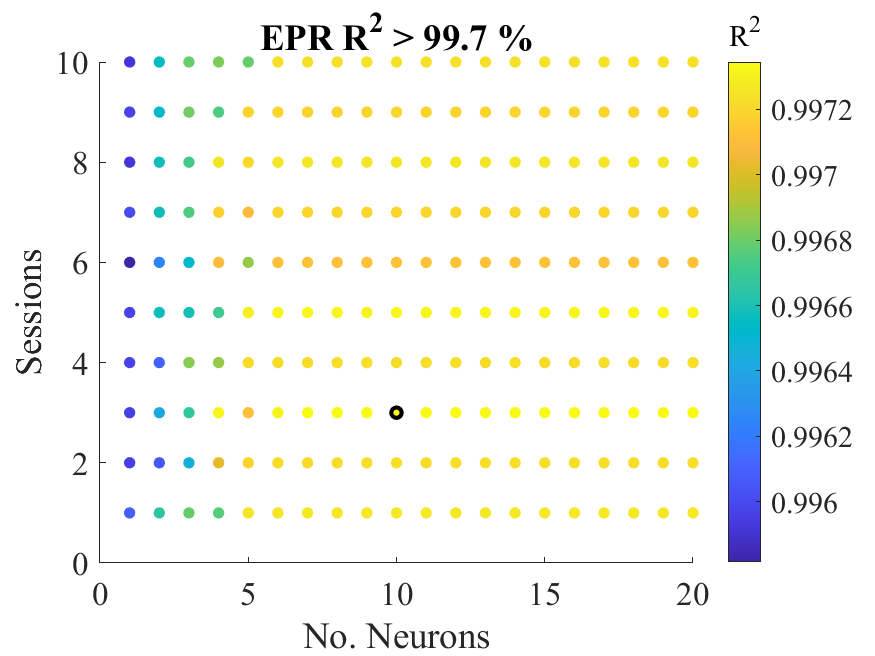
\includegraphics[width=\textwidth]{EPRR2TrialsNeurons.png}
        \caption{}
        \label{fig:TrialsNeuronsEPR}
    \end{subfigure}
\begin{subfigure}[b]{0.49\textwidth}
	\centering
	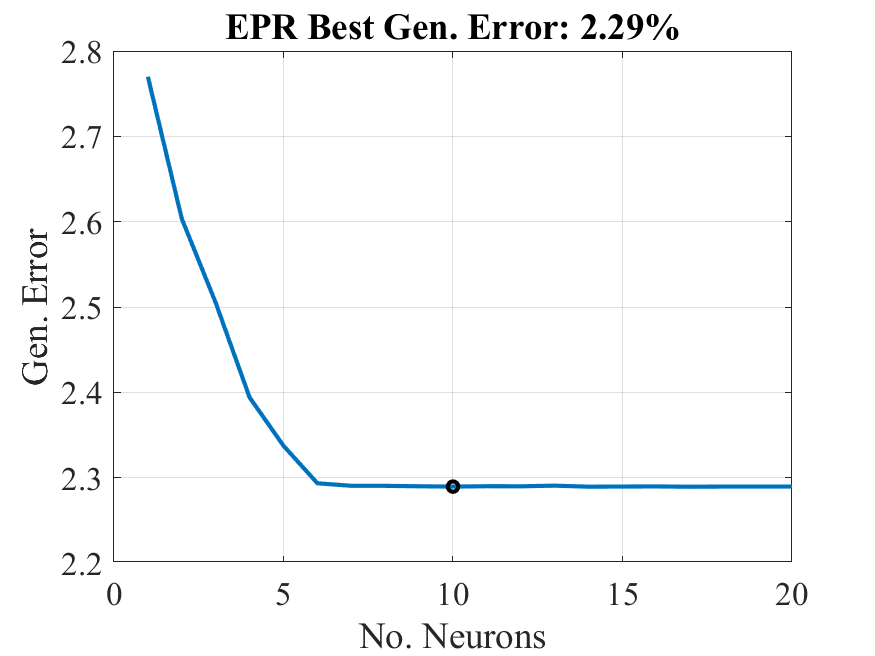
\includegraphics[width=\textwidth]{EPRGeNeurons.png}
	\caption{}
	\label{fig:GenNeuronsEPR}
\end{subfigure}
    
    \begin{subfigure}[b]{0.49\textwidth}
        \centering
        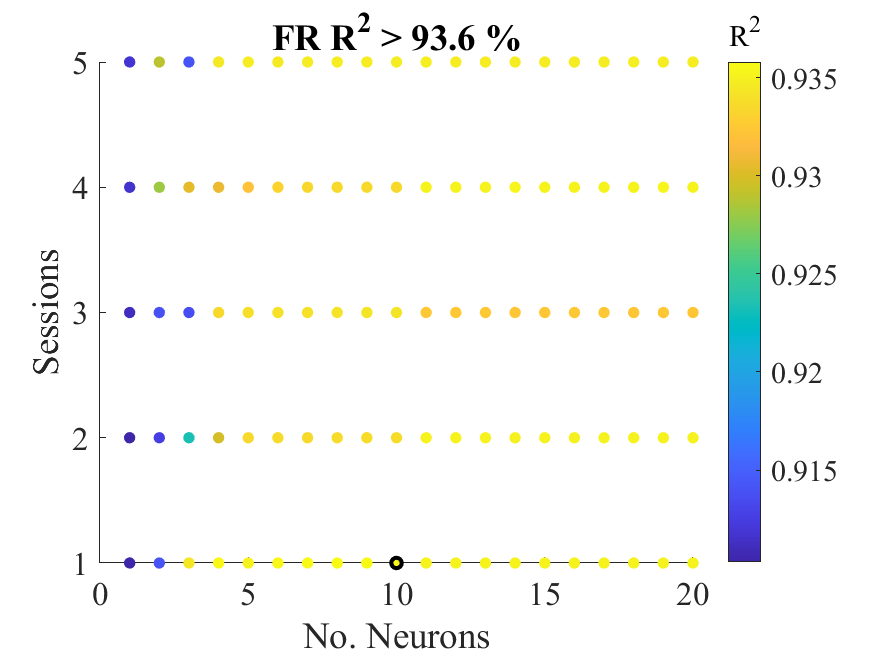
\includegraphics[width=\textwidth]{FRR2TrialsNeurons.png}
        \caption{}
        \label{fig:TrialsNeuronsFR}
    \end{subfigure}
\begin{subfigure}[b]{0.49\textwidth}
	\centering
	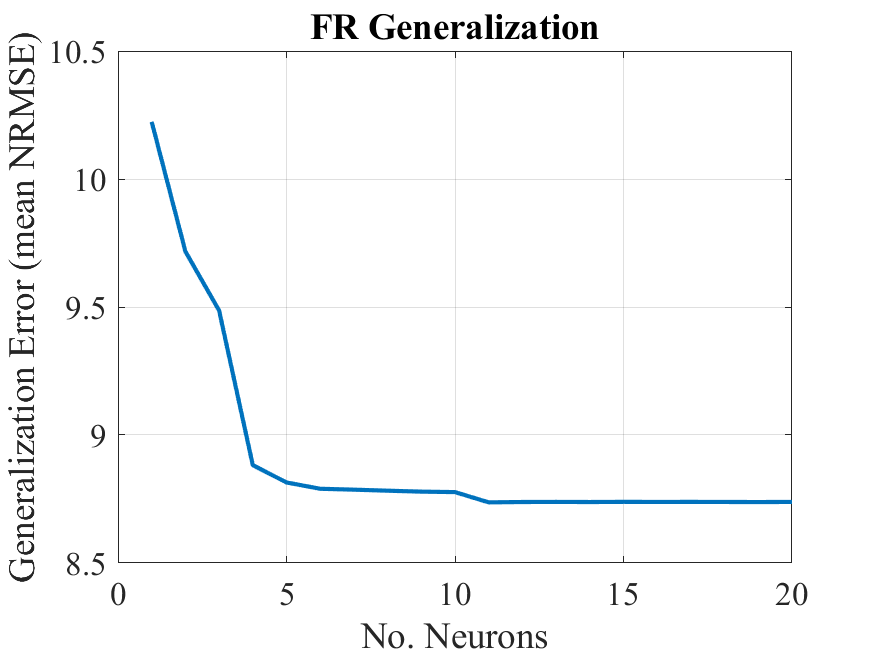
\includegraphics[width=\textwidth]{FRGeNeurons.png}
	\caption{}
	\label{fig:GenNeuronsFR}
\end{subfigure}
    
    \begin{subfigure}[b]{0.49\textwidth}
        \centering
        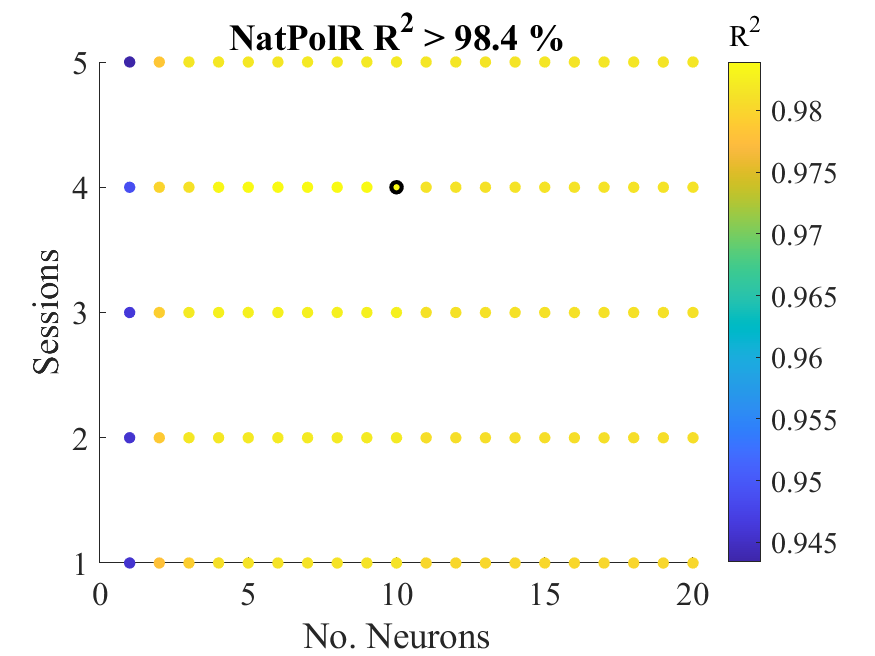
\includegraphics[width=\textwidth]{NatPolRR2TrialsNeurons.png}
        \caption{}
        \label{fig:TrialsNeuronsNatPolR}
    \end{subfigure}
\begin{subfigure}[b]{0.49\textwidth}
	\centering
	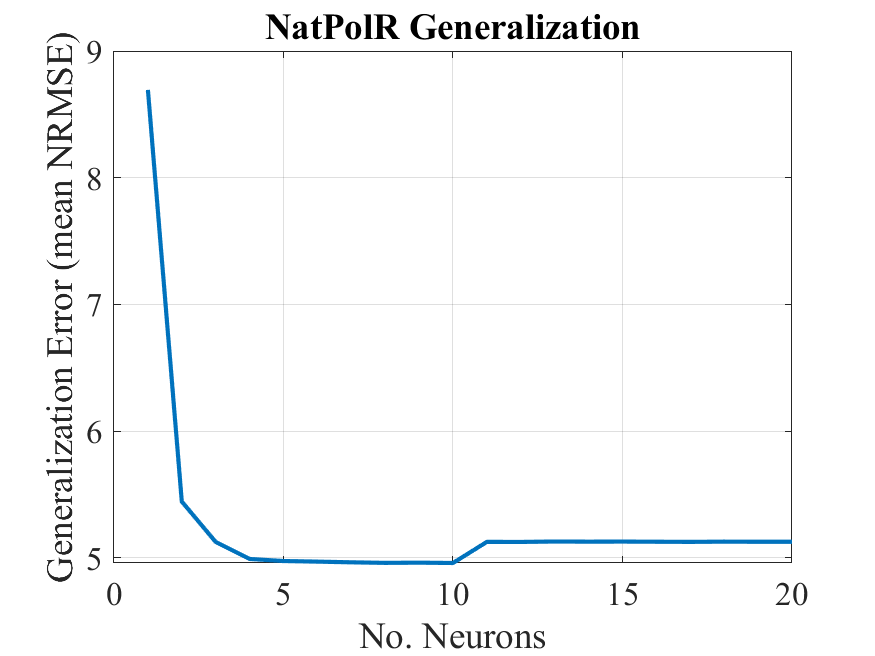
\includegraphics[width=\textwidth]{NatPolRGeNeurons.png}
	\caption{}
	\label{fig:GenNeuronsNatPolR}
\end{subfigure}
    \caption{Impact of the number of neurons on the $R^2$ value (a), (c), (e), and the Generalization error (b), (d), (f), for the EPR, FR, and NatPolR materials. A total of 200 ANN models are trained per soft material. The best $R^2$ value is circled in (a), (c), (e). The optimal number of neurons is circled in (b), (d), (f).}
    \label{fig:TrialsNeurons1}
\end{figure}

\begin{figure}[htbp!]
	\centering
    
    \begin{subfigure}[b]{0.49\textwidth}
        \centering
        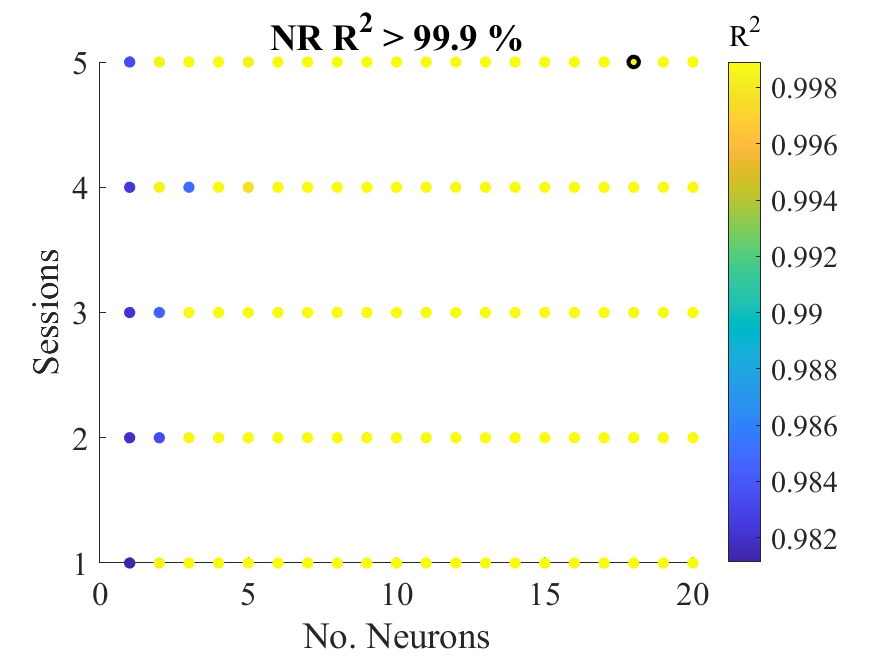
\includegraphics[width=\textwidth]{NRR2TrialsNeurons.png}
        \caption{}
        \label{fig:TrialsNeuronsNR}
    \end{subfigure}
\begin{subfigure}[b]{0.49\textwidth}
	\centering
	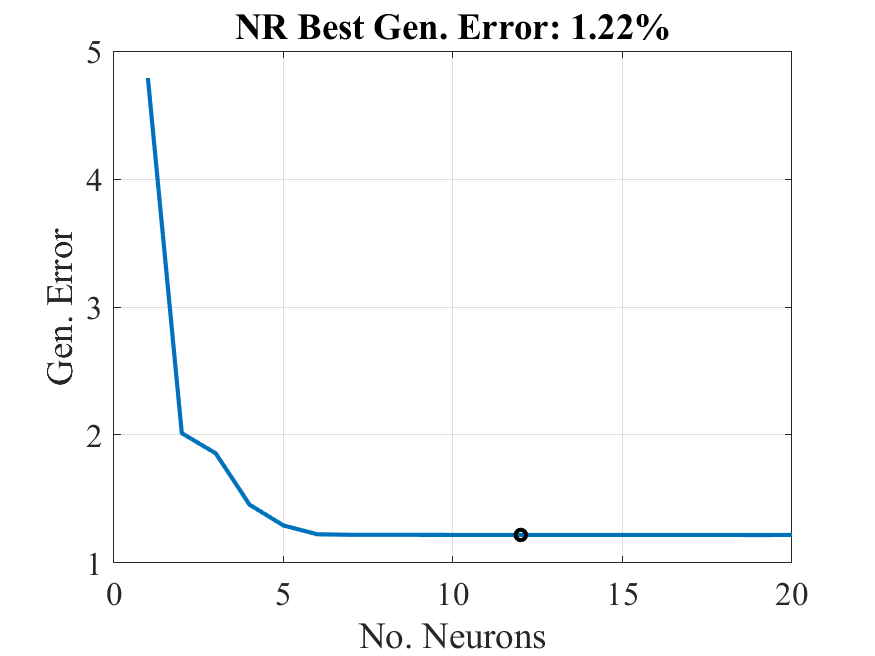
\includegraphics[width=\textwidth]{NRGeNeurons.png}
	\caption{}
	\label{fig:GenNeuronsNR}
\end{subfigure}
    
    \begin{subfigure}[b]{0.49\textwidth}
        \centering
        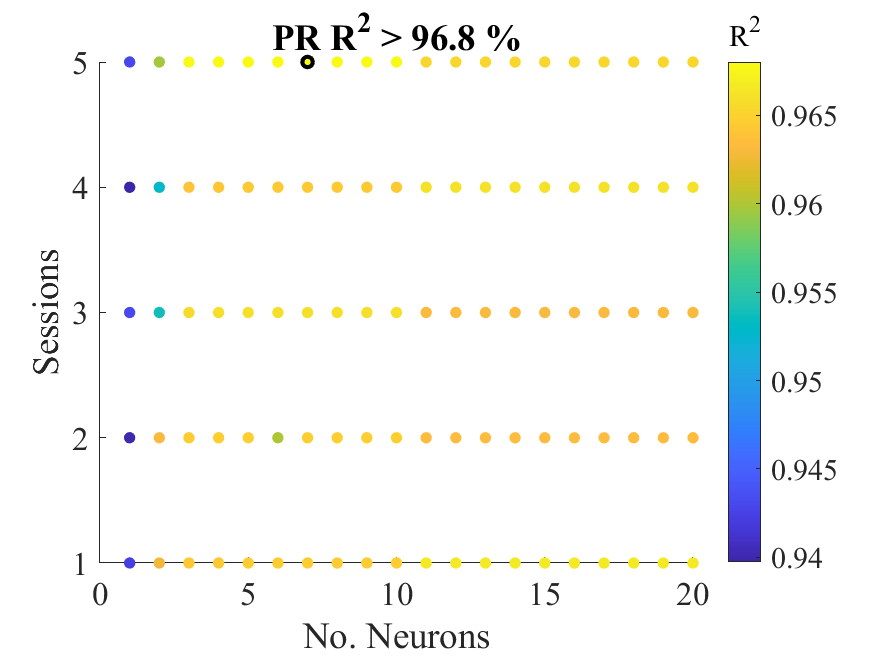
\includegraphics[width=\textwidth]{PRR2TrialsNeurons.png}
        \caption{}
        \label{fig:TrialsNeuronsPR}
    \end{subfigure}
\begin{subfigure}[b]{0.49\textwidth}
	\centering
	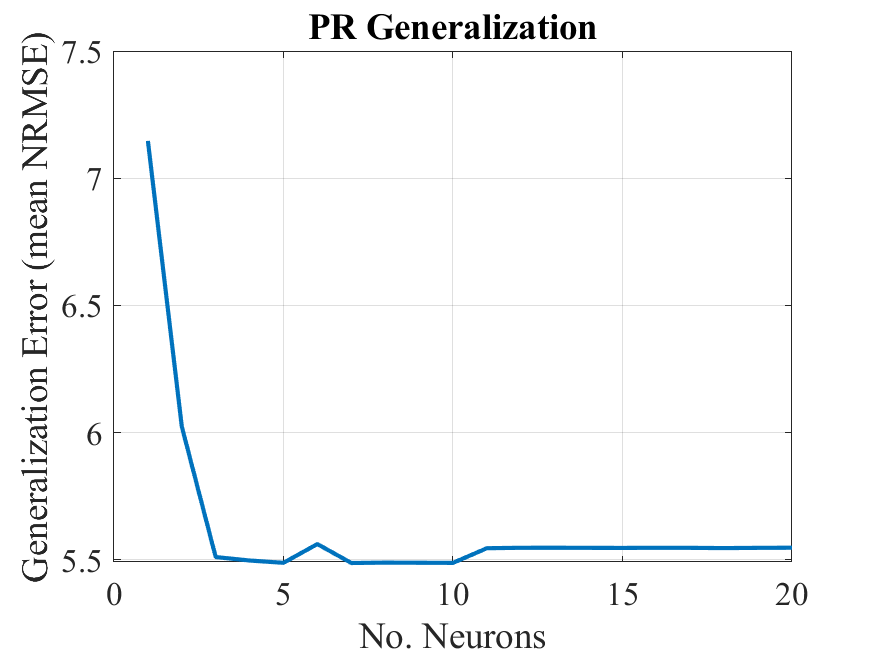
\includegraphics[width=\textwidth]{PRGeNeurons.png}
	\caption{}
	\label{fig:GenNeuronsPR}
\end{subfigure}
    
    \begin{subfigure}[b]{0.49\textwidth}
        \centering
        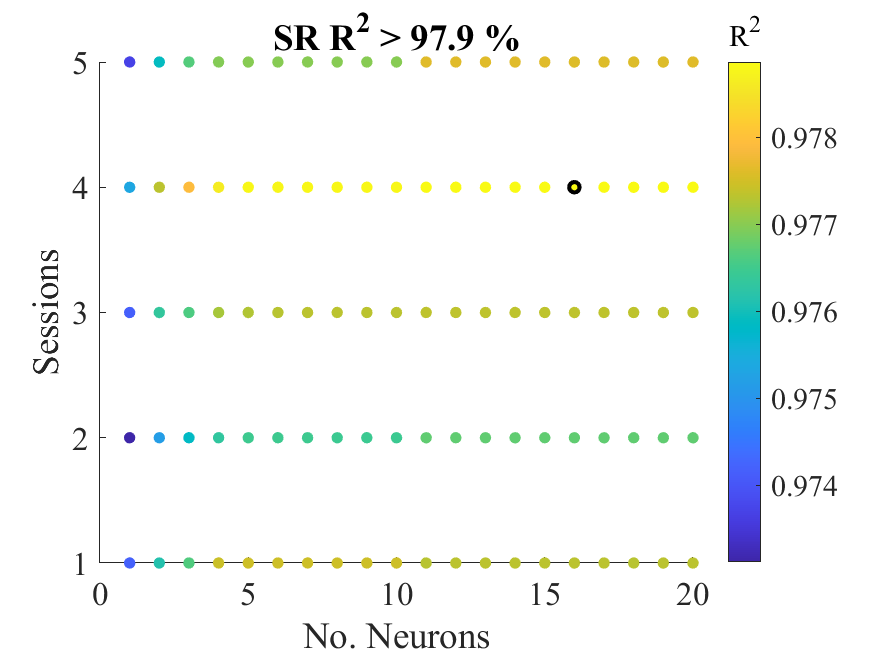
\includegraphics[width=\textwidth]{SRR2TrialsNeurons.png}
        \caption{}
        \label{fig:TrialsNeuronsSR}
    \end{subfigure}
\begin{subfigure}[b]{0.49\textwidth}
	\centering
	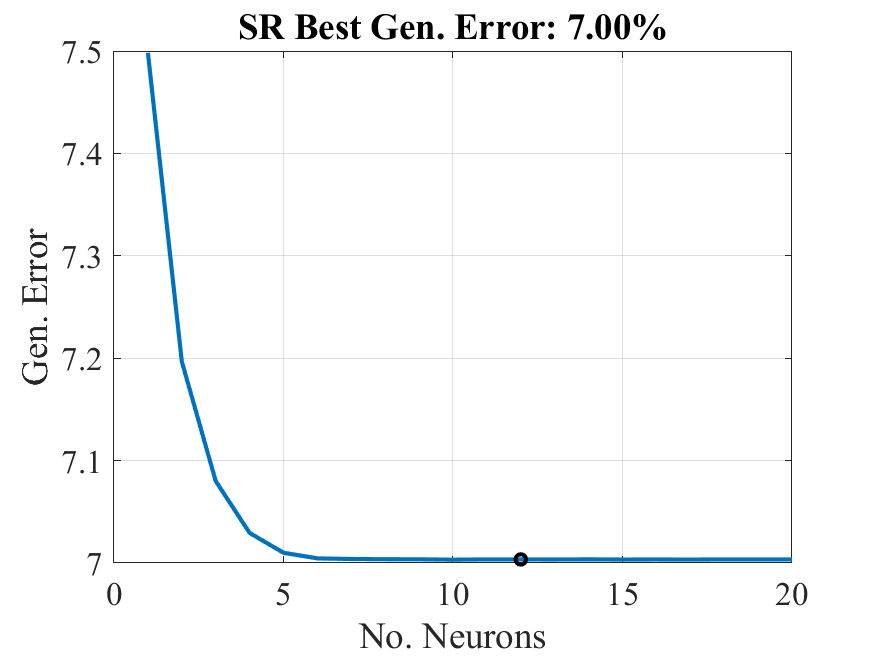
\includegraphics[width=\textwidth]{SRGeNeurons.png}
	\caption{}
	\label{fig:GenNeuronsSR}
\end{subfigure}
    \caption{Impact of the number of neurons on the $R^2$ value (a), (c), (e), and the Generalization error (b), (d), (f), for the NR, PR, and SR materials. A total of 200 ANN models are trained per soft material. The best $R^2$ value is circled in (a), (c), (e). The optimal number of neurons is circled in (b), (d), (f).}
    \label{fig:TrialsNeurons2}
\end{figure}

\begin{figure}[htbp!]
	\centering    
    \begin{subfigure}[b]{0.49\textwidth}
        \centering
        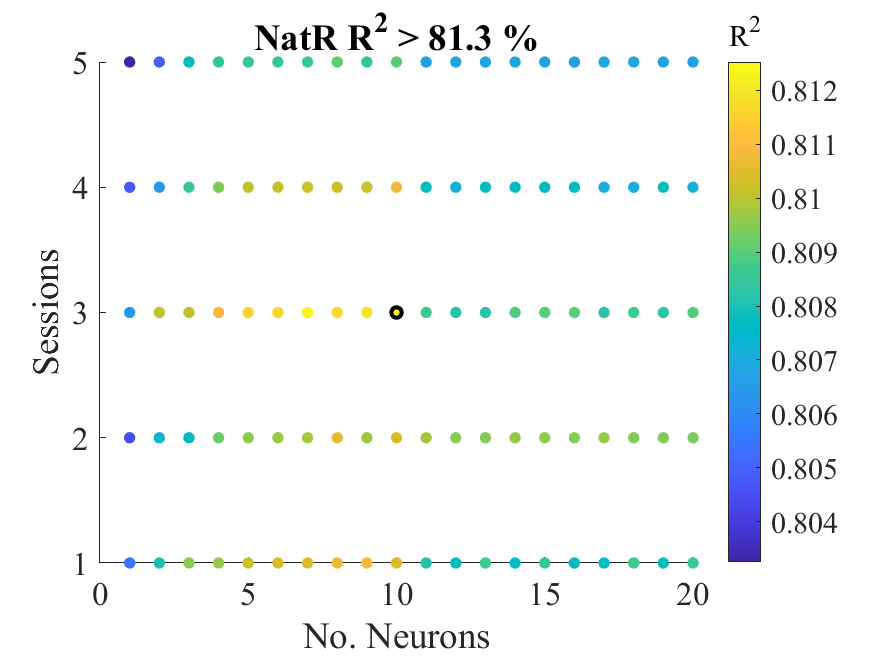
\includegraphics[width=\textwidth]{NatRR2TrialsNeurons.png}
        \caption{}
        \label{fig:TrialsNeuronsNatR}
    \end{subfigure}
	\begin{subfigure}[b]{0.49\textwidth}
		\centering
		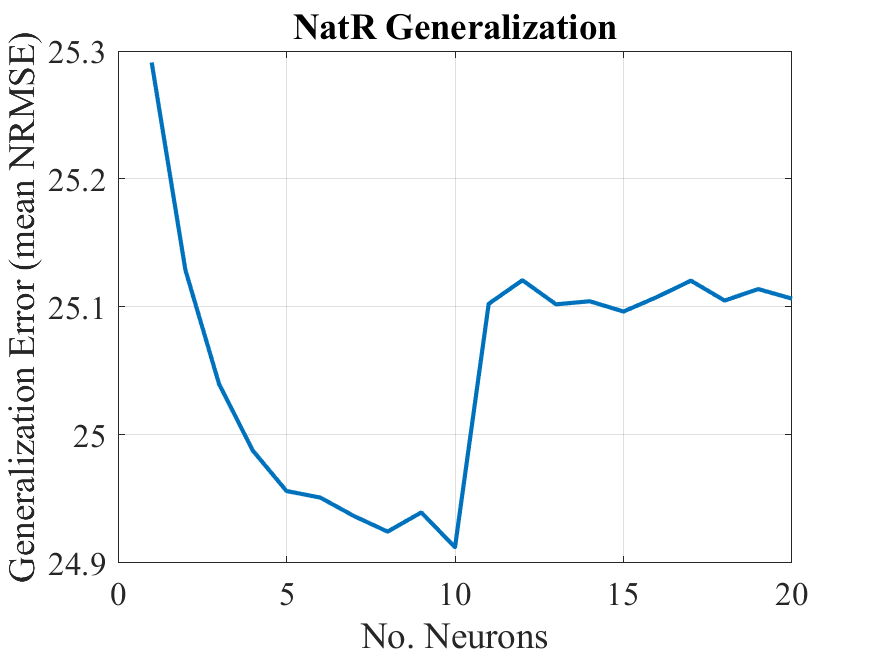
\includegraphics[width=\textwidth]{NatRGeNeurons.png}
		\caption{}
		\label{fig:GenNeuronsNatR}
	\end{subfigure}
    \caption{Impact of the number of neurons on the $R^2$ value (a) and the Generalization error (b), for the NatR material. A total of 200 ANN models are trained per soft material. The best $R^2$ value is circled in(a). The optimal number of neurons is circled in (b).}
    \label{fig:TrialsNeurons3}
\end{figure}


The achieved generalization errors (Gen. Error) and the $R^2$ values obtained from this optimization are illustrated in \Cref{fig:TrialsNeurons1,fig:TrialsNeurons2,fig:TrialsNeurons3}. The calculation of the Gen. Error is based on the mean value of the NRMSE values obtained during the 10 training sessions, as follows:

\begin{equation}
\label{eqGenError}
Gen. Error = \frac{1}{N}\sum_{j=1}^{N} NRMSE_j
\end{equation}

\noindent where $N$ is the total number of training sessions, 10, and the subscript $j$ represents the $NRMSE$ value obtained in each individual training session. It is important to mention that the training set is different from one training session to the other, but it is constant among the different number of neurons tested.

The $R^2$ value, or coefficient of determination, indicates the fraction of the data variation which is explained by the ANN models. Traditionally, a $R^2$ value closer to 1 indicates a very good model fit. However, in the field of ANNs, a very high $R^2$ value could actually indicate over-fit in the developed ANN. In general, most of the achieved $R^2$ values are below the desired threshold of $R^2>99.9\%$. Only the ANN model NR material is able to meet the latter threshold. In contrast, the lowest $R^2$ value achieved among all materials is reported for the NatR material as $R^2>81.6\%$. 

The ANN models with the optimal number of neurons must have the right combination of good accuracy (small NRMSE), low number of neurons, and high $R^2$ values. The first parameter to consider is the $R^2$ value. For the training sessions with a $R^2 > 99.9\%$, the optimal candidate is the one with the lowest number of neurons. For the cases in which the threshold is not achieved, the maximum achieved  $R^2$ value is taken as reference. Following these conditions, the optimal number of neurons per soft material are extracted and presented in \Cref{tbl:ANNvsSLS}. In here, the PL-SLS and the PL-Wiechert models are also compared against the developed ANN model.

\begin{table}[htb!]
	\centering
	\caption{Comparison between the performance of the best case ANN model, the PL-SLS model, and the PL-Wiechert model. The generalization error, Gen. Error \Cref{eqGenError}, is based on the mean NRMSE value from all training sessions, whereas the $GE$ \Cref{eqGE}, is based on the mean NRMSE among all available strain rates as described in \Cref{sec:ChapterModellingLVM}.}
	\begin{tabular}{p{1em} l ccccccc}
		\toprule
		&                   				& EPR   & FR    & NatPolR	& NR  & PR    & SR    & NatR\\
		\hline
		\multicolumn{9}{l}{ANN model}\\
			&Gen. Error (\%)          			& 2.29  & 8.75  & 5.04		& 1.22  & 5.48  & 7     &   24.9\\
		&$R^2$             					& 99.7 	& 93.6	& 98.5		& 99.9	& 96.9	& 97.9	&   81.6\\	
		&No. of Neurons                     & 10    & 17    & 13	   	& 12    & 5     & 12    &   10\\
		
		\hline
		\multicolumn{9}{l}{PL-SLS model}\\
		&$GE$ (\%)          				& 13.04	& 3.03  & 2.27		& 1.36  & 2.70  & 1.44	& 1.10\\
		&Tolerance (\%)                 	& 60  	& 90    & 30    	& 40    & 40    & 70    & 80\\
		\hline
		\multicolumn{9}{l}{PL-Wiechert model}\\
		&$GE$ (\%)          & 10.34    & 4.44  & 2.51   & 2.36  & 3.64  & 0.55   & 1.12\\
		&Tolerance (\%)                 & 90    & 70    & 10    & 70    & 60    & 60    & 80\\		
		\bottomrule
	\end{tabular}
	\label{tbl:ANNvsSLS}
\end{table}

The values of the generalization error for all the three models are very similar. The calculation of this parameter is different between the ANN models \Cref{eqGenError} and the PL models \Cref{eqGE}. Nonetheless, in both cases, the generalization error measures the capabilities of the models for accounting the non-linear velocity-dependent stress response of the studies soft materials.

In general, the generalization error values of the developed ANN models are slightly higher then the values reported for the PL models. This is expected due to the selection criteria when choosing the optimal number of neurons. In other words, this is the potential effect of constraining the number of neurons to avoid over-fitting from happening. Nonetheless, the NatR material is identified as an outlier. This material reported a significantly different Gen. Error value of 24.9\% which is also not aligned with the generalization errors reported for the PL models. The potential cause of this is the uneven dataset available for this material in which much of the data is concentrated in the strain rates of 250 and 500 mm/min. Another potential cause of this is the limited number of neurons used, in comparison to the size of the dataset available for this soft material, which is the largest among all the studied materials. This hypothesis is further verified by looking at \Cref{fig:ANNGenNatR} from the selection of inputs optimization where only 10\% of the whole dataset is used. In this scenario, the Gen. Error achieved by the ANN model is around 5\%, a value closer to the Gen. Error values reported in \Cref{tbl:ANNvsSLS}.

Interestingly enough, the ANN models performed better for the case of the EPR material, where the PL models performed the worst. Again, this can be related to the characteristics of the dataset. For this material, there is no available data for the strain rate of 250 mm/min. In addition to this, the stress-strain curves of this material for the strain rates of 50 and 250 mm/min are very similar (\Cref{sfig:EPRSS}). Due to this, a small Gen. Error in this scenario could in fact indicate over-fitting. Nonetheless, the developed ANN models performed better than Std. Lin. SDS model, the reference which has been used along this thesis, where the reported relative RMSE is of 13.6\%. Therefore, the developed ANN models are also suitable for the prediction of the non-linear, time dependent, and strain dependent stress response of viscoelastic materials. Lastly, the performance of the developed ANN models is further validated under simulated real-time conditions, replicating as much as possible the conditions expected in a real robotic application.

\section{Summary}

%this work \cite{xu2019artificial} an ANN which accounts for the strain rate of the materials is trained with three different strain rates. The trained and validated ANN was used to predict the elastic modulus of the materials under unknown strain rates. 

In this chapter, a feedforward artificial neural network model is developed and tested as an alternative to traditional modelling approaches based on the LVMs, such as the PL models developed in \Cref{sec:ChapterModellingLVM}, which can be very computationally costly. Artificial neural networks have been successfully implemented is many applications, but the literature available on the prediction of the viscoelastic properties of soft materials is still scarce. The developed ANN models are aimed to be used in real robotics applications, specifically to predict the mechanical behaviour of the viscoelastic element found in a recent actuation technology, the series-viscoelastic actuator.

The process of developing the ANN models involved the optimization of the number of neurons in the hidden layer and the most appropriate selection of inputs and outputs, to account for the viscoelastic properties of the studied soft materials. The optimal number of neurons varied from one material to the other but it does not exceed 20 neurons. The inputs of the ANN models are defined as the strain and the strain rate of the materials. As the output, the ANN models are aimed to predict the stress response. In order to avoid over-fitting, the Bayesian Regularization algorithm is used instead of a traditional early stopping method such as the Levenberg-Marquardt algorithm.

The generalization capabilities of the ANN models are assessed using a k-fold cross validation approach together with multiple training sessions. In this way, the network is trained and tested with unique data subsets in each training sessions. The mean NRMSE from these training sessions is defined as the generalization error of the ANN models. In general the ANN models outperformed the Std. Lin. SDS model documented in the literature, which has been used as reference in this thesis. When comparing the performance of the ANN models to the PL models, two outliers are detected. On the one hand, the ANN model for the EPR material outperformed the developed PL models. On the other hand, the ANN model for the NatR material performed worse than the PL models. The differences in performances could be caused by the characteristics of the dataset of each of these materials. This however, do not disregard the capabilities of the ANN models to account for the non-linear velocity-dependent stress response of soft materials. Nonetheless, the performance of these modelling approaches when being implemented as part of a control system is still unknown. This is investigated in the following chapter.